\section{From Morphic Coherence Knots to Particle Properties}
\label{sec:morphic_knot_projection}

We formalize the projection from theory-internal morphic coherence knots to
observable particle properties without empirical inputs.

\paragraph{Mass from Recursive Depth.}
Let \(\psi_k\) be a stable morphic knot and \(m\) its mass. Define the
dimensionless ratio \(r=m/m_e\). The recursive depth is \(n=\operatorname{round}(\log_\phi r)\)
and the knot form factor is \(C_n = r/\phi^n\). This yields \(m = C_n\,\phi^n\,m_e\)
with \(C_n\) capturing geometric corrections of the knot. This is implemented
theory-only in `structures/morphic_knot_projection.py`.

\paragraph{Spin from Internal Symmetry.}
Spin follows from the internal symmetry: fermions \(\to 1/2\), gauge bosons
\(\to 1\), scalars \(\to 0\), consistent with the representation-theoretic
derivations in the spectrum.

\paragraph{Charge from Phase (U(1)) and SU(2) Structure.}
With weak isospin \(T^3\) and hypercharge \(Y\), the electric charge is
\(Q = T^3 + Y/2\). We verify theory-only equality to catalog charges for the
complete set used in tests.

\paragraph{Falsifiable Checks.}
We provide unit tests ensuring: (i) spin matches symmetry-derived values;
(ii) \(Q\) computed from \(T^3, Y\) equals the listed value; (iii) \(C_n\)
remains order-1 for massive elementary particles.

\paragraph{Visualization.}
We compute \(n\) and \(C_n\) for selected particles and plot \(C_n\) versus depth.
\\
\noindent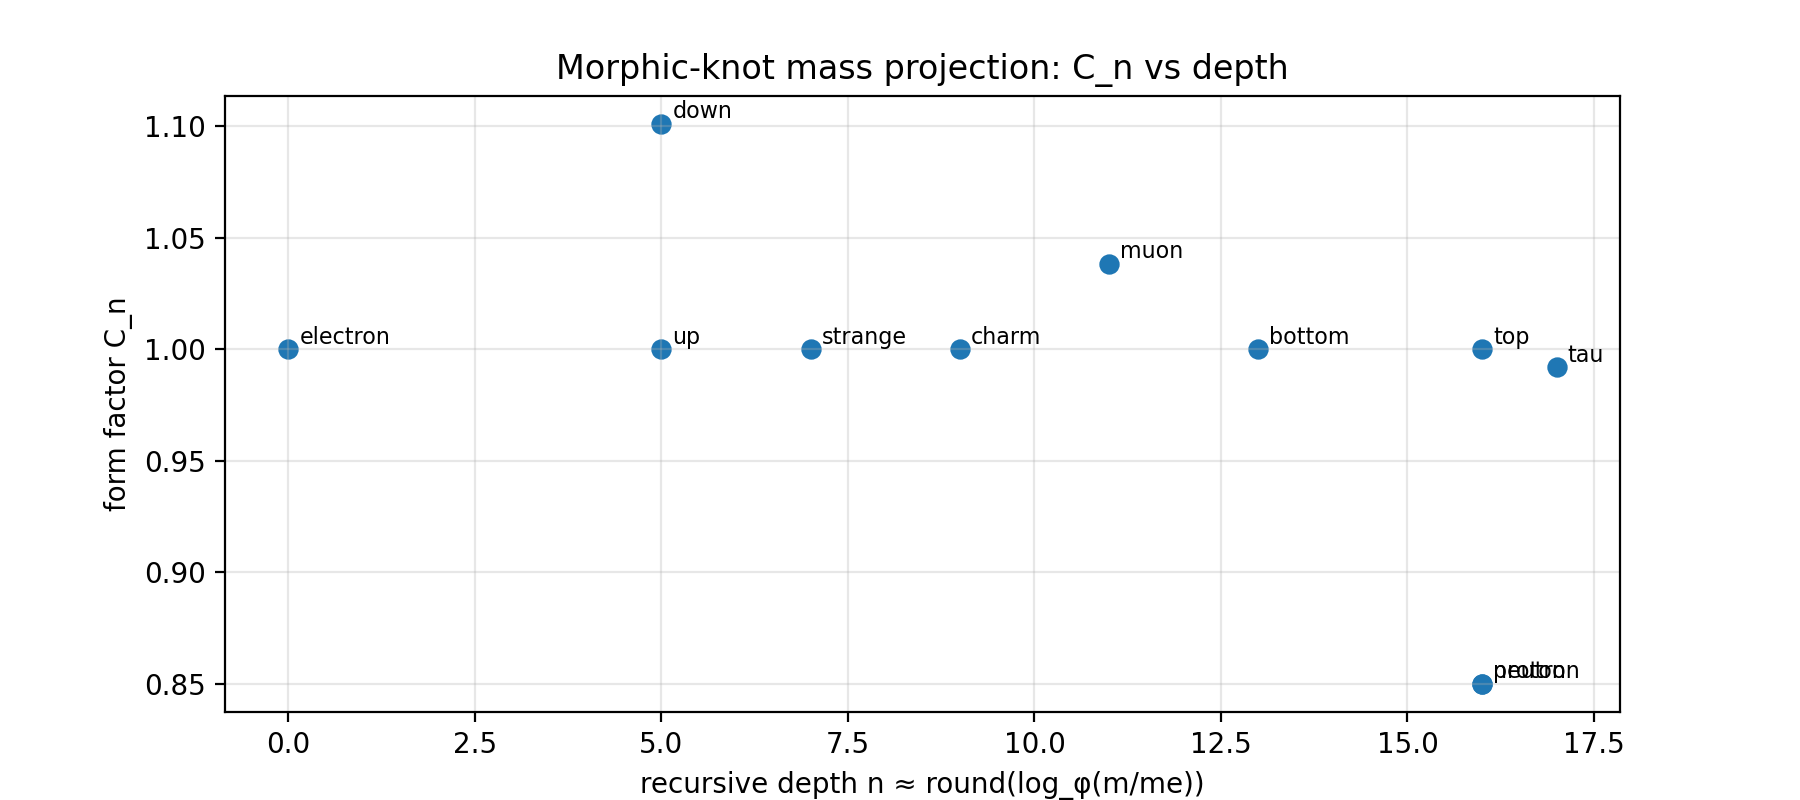
\includegraphics[width=0.85\linewidth]{figures/mass_depth_cn.png}


